%% LyX 2.2.1 created this file.  For more info, see http://www.lyx.org/.
%% Do not edit unless you really know what you are doing.
\documentclass[english]{article}
\usepackage[T1]{fontenc}
\usepackage[latin9]{inputenc}
\usepackage{geometry}
\geometry{verbose}
\usepackage{array}
\usepackage{multirow}
\usepackage{amsmath}
\usepackage{graphicx}

\makeatletter

%%%%%%%%%%%%%%%%%%%%%%%%%%%%%% LyX specific LaTeX commands.
%% Because html converters don't know tabularnewline
\providecommand{\tabularnewline}{\\}

%%%%%%%%%%%%%%%%%%%%%%%%%%%%%% User specified LaTeX commands.
\usepackage{cite}
\usepackage[T1]{fontenc}
\usepackage{inputenc}
\usepackage{authblk}
\usepackage{lmodern}
\author[1,2]{Daniel Schlauch} 
\author[3]{Heide Fier}
\author[1,2]{Christoph Lange}
\affil[1]{Department of Biostatistics, Harvard TH Chan School of Public Health, Boston, MA 02115}
\affil[2]{Department of Biostatistics and Computational Biology, Dana-Farber Cancer Institute, Boston, MA 02115}
\affil[3]{Institute of Genomic Mathematics, University of Bonn, Bonn, Germany}

\makeatother

\usepackage{babel}
\begin{document}

\title{On the detection of genetic heterogeneity in whole-genome sequencing
studies: A statistical test for the identification of \textquotedblleft genetic
outliers\textquotedblright{} due to population sub-structure or cryptic
relationships}
\maketitle
\begin{abstract}
In order to minimize the effects of genetic confounding on the analysis
of high-throughput genetic association studies, e.g. (whole-genome)
sequencing studies, genome-wide association studies (GWAS), etc.,
we propose a general framework to assess and to test formally for
genetic heterogeneity among study subjects. Even for relatively moderate
sample sizes, the proposed testing framework is able to identify study
subjects that are genetically too similar, e.g cryptic relationships,
or that are genetically too different, e.g. population substructure.
The approach is computationally fast, enabling the application to
whole-genome sequencing data, and straightforward to implement. Simulation
studies illustrate the overall performance of our approach. In an
application to the 1000 genomes project, we outline an analysis/cleaning
pipeline that utilizes our approach to formally assess whether study
subjects are related and whether population substructure is present.
In the analysis of 1000 Genomes Project, our approach revealed studies
subjects that are most likely related, but have passed so far standard
qc-filters. An implementation of our method, Similarity Test for Estimating
Genetic Outliers (STEGO), is available in the R package \textbf{stego}
from Github at https://github.com/dschlauch/stego.
\end{abstract}

\section*{Author Summary}

In analyses of genetic data, it is critical to have a precise understanding
of the relationships between individuals in the study including identification
of individuals who are related as well as complex structure arising
from differing ancestral histories. Incomplete information on these
features may confound association studies, leading to both increased
Type I and Type II errors. Many methods have been developed to address
these problems, but do not specifically utilize each variant's allele
frequency as an informative value. As sequencing technology becomes
more available, the information captured in rarer alleles allows us
a more precise measure of the relationships between individuals. Here,
we present a formal statistical measure of similarity in the context
of genetic studies which has far reaching utility in quantifying population
homogeneity and adjustment in association analyses. We demonstrate
that our approach can be used to detect such features as population
structure and cryptic relatedness in a powerful and statistically
rigorous manner. These claims are tested using data from all 26 populations
in the 1000 Genomes Project, which revealed previously undocumented
differing levels of genetic heterogeneity and cryptic relatedness
across the groups. 

\section*{Introduction}

The fundamental assumption in standard genetic association analysis
is that the study subjects are independent and that, at each locus,
the allele frequency is identical across study subjects\cite{choi2009case,purcell2007plink,yang2010common}.
In the presence of population heterogeneity, e.g. population substructure
or cryptic relatedness, these assumptions are violated. It can introduce
confounding into the analysis and lead to biased results, e.g. false
positive findings\cite{price2006principal,kang2010variance,ptak2002evidence,voight2005confounding}.
Given the generality of the problem, it has been the focus of methodology
research for a long time. For candidate gene studies and later genome-wide
association studies (GWAS), genomic control was developed\cite{devlin2001genomic,bacanu2002association}.
The approach adjusts the association test statistics at the loci of
interest by an inflation factor that is estimated at a set of known
null-loci. With the arrival of GWAS data, it became possible to estimate
the genetic dependence between study subjects and the overall genetic
variation for each study subject by computing the empirical genetic
variance/covariance matrix between study subjects at a whole genome
level. The genetic variance/covariance matrix can then be utilized
in two ways to minimize the effects of population substructure on
the association analysis. 

The first method is to compute an eigendecomposition of the matrix
and to include the eigenvectors that explain the most variation as
covariates in the association analysis\cite{price2006principal,price2010new}.
An alternative approach is to incorporate the estimated dependence
structure of the study subjects directly into a generalized linear
model and account so directly for the dependence at the model-level\cite{listgarten2012improved,lippert2011fast,zhang2010mixed}.
Both approaches have proven to work well in numerous applications.
While the first approach is computationally fast and easy to implement,
the direct modeling of the dependence structure between study subjects
can be more efficient. 

However, both approaches benefit if, prior to the analysis, study
subjects whose genetic profile is very different from the other study
subjects, e.g. \textquotedblleft genetic outliers\textquotedblright ,
are removed from the data set. The standard practice is currently
to examine the eigenvalue plots visually and to identify outliers
by personal judgment on how far study subjects are from the \textquotedblleft clouds\textquotedblright{}
of study subjects. As typically up to 10 eigenvectors have to be considered,
this process of identifying outliers can become a complicated and
subjective procedure. 

Many methods for exist for inferring relatedness which make the strong
assumption of population homogeneity\cite{purcell2007plink,yang2010common,kang2010variance,choi2009case}.
These methods have been shown to be biased in the context of population
heterogeneity \cite{manichaikul2010robust}. More recently, methods
have been developed recently which attempt to estimate relatedness
with population structure \cite{thornton2012estimating,manichaikul2010robust}.
These developments improve the ability to detect existing pedigrees,
which can aid in the removal of individuals who violate homogeneity.
However, there is currently no quantitative measure of homogeneity
which can be used to test a dataset prior to the application of GWAS.

In this communication, we propose a formal statistical test that assesses
whether two study subjects come from the same population and whether
they are unrelated. The test statistic is based on an adaptation of
the Jaccard Index which utilizes the idea that variants are differentially
informative of relatedness based on their allele frequency. Recent
work has shown that the Jaccard Index alone can be used to reveal
finer scale population structure compared with existing methods such
as EIGENSTRAT\cite{prokopenko2016utilizing}. Furthermore, the distribution
of our statistic can be derived under the null-hypothesis which makes
it computationally fast, enabling the application to whole-genome
sequencing data. Our measure has clearly defined properties which
can be used to test for homogeneity in a population and in particular
identify individuals who are likely be related in a study population.
Applications to the 1,000 Genome Project suggests that our approach
is better suited to detect sub-populations than genetic variance/covariance
approach. This is most likely attributable to the emphasis of our
approach on small allele frequencies.

\section*{Methods}

Exploiting the information in rare variants (RVs), such as one with
minor allele frequency (MAF) < 1\%, is fundamental to our method,
as our approach utilizes the features of RVs that they are typically
more recent than common variants and that many of them are population/family
specific. Since allele frequencies can differentially confound association
studies \cite{mathieson2012differential}, we developed a method that
utilizes the differential informativeness of variants by allele frequency
to obtain a high resolution picture of population structure and protect
the association study against bias due to genetic confounding. Our
approach uses an intuitive, computationally straightforward approach
towards identifying similarity between two study subjects which is
also directly linked to the kinship coefficient. 

\subsection*{Similarity measure among haploid genomes}

Consider a matrix of $n$ individuals ($2n$ haploid genomes), with
$N$ independent variants described by the genotype matrix $\mathbf{G}_{2n\times N}$.
$\mathbf{G}$ is a binary matrix with value $1$ indicating the presence
of the minor allele and $0$ indicating the major allele. We define
the similarity index between two haploid genomes, $s_{i,j}$

\begin{equation}
s_{i,j}=\frac{\sum_{k=1}^{N}w_{k}\mathbf{G}_{i,k}\mathbf{G}_{j,k}}{\sum_{k=1}^{N}I\left[\sum_{l=1}^{2n}\mathbf{G}_{l,k}>1\right]}\label{eq:s equation}
\end{equation}

where 

\[
w_{k}=\begin{cases}
\frac{{2n \choose 2}}{{\sum_{l=1}^{2n}\mathbf{G}_{l,k} \choose 2}} & \sum_{l=1}^{2n}\mathbf{G}_{l,k}>1\\
0 & \sum_{l=1}^{2n}\mathbf{G}_{l,k}\le1
\end{cases}
\]

In the absence of population structure, i.e. homogeneous population
we have
\begin{align*}
E\left(s_{i,j}\right) & =1
\end{align*}

It therefore follows from the Central Limit Theorem that in the absence
of population structure, cryptic relatedness and dependence between
loci (such as linkage disequilibrium) the distribution of the similarity
index, $s_{i,j}$ is Gaussian.
\[
s_{i,j}\sim N\left(1,\sigma_{i,j}^{2}\right)
\]
Where the variance of $s_{ij}$ can be estimated by 
\begin{equation}
\hat{\sigma_{i,j}^{2}}=\hat{Var}\left(s_{i,j}\right)=\frac{\sum_{k=1}^{N}\left(w_{k}-1\right)}{\left(\sum_{k=1}^{N}I\left[\sum_{l=1}^{2n}\mathbf{G}_{l,k}>1\right]\right)^{2}}\label{eq: variance equation}
\end{equation}

The similarity index $s_{i,j}$ provides an easily interpreted statistical
test for evaluating possible relatedness between individuals in a
purportedly homogeneous dataset of unrelated individuals. Note that
this formulation is independent of the samples $i,j$ and depends
only on the allele counts for each variant across the study group.
See Supplemental Methods.

\subsection*{Similarity measure among diploid genomes}

This approach is easily generalized to the diploid scenario. A diploid
similarity score, $s_{diploid}$, is obtained by averaging each of
the four pairwise haploid $s_{haploid}$ scores between each person's
two haploid genotypes. For $n$ individuals, $2n$ genotypes per locus,
the similarity between individuals $i$ and $j$ is defined as

\[
s_{i,j}^{\left(diploid\right)}=\frac{\sum_{k=1}^{N}\left[w_{k}\mathbf{G}_{i_{1},k}\mathbf{G}_{j_{1},k}+w_{k}\mathbf{G}_{i_{1},k}\mathbf{G}_{j_{2},k}+w_{k}\mathbf{G}_{i_{2},k}\mathbf{G}_{j_{1},k}+w_{k}\mathbf{G}_{i_{2},k}\mathbf{G}_{j_{2},k}\right]/4}{\sum_{k=1}^{N}I\left[\left(\sum_{l=1}^{n}\left[\mathbf{G}_{l_{1},k}+\mathbf{G}_{l_{2},k}\right]\right)>1\right]}
\]

\[
s_{i,j}^{\left(diploid\right)}=\frac{\sum_{k=1}^{N}\sum_{l=1}^{2}\sum_{m=1}^{2}\left[w_{k}\mathbf{G}_{i_{l},k}\mathbf{G}_{j_{m},k}\right]/4}{\sum_{k=1}^{N}I\left[\left(\sum_{l=1}^{n}\left[\mathbf{G}_{l_{1},k}+\mathbf{G}_{l_{2},k}\right]\right)>1\right]}
\]
where $\mathbf{G}_{i_{2},k}$ refers to the $2^{nd}$ genotype of
individual $i$ at locus $k$.

Here it becomes clear that the method can be applied to phased and
unphased data alike. For an unphased data matrix $\mathbf{H}_{n\times N}$,
where $\mathbf{H}$ contains the number of minor alleles, $\left\{ 0,1,2\right\} $,
for a subject at a particular variant. 
\[
s_{i,j}^{\left(diploid\right)}=\frac{\sum_{k=1}^{N}\left[w_{k}\mathbf{H}_{i,k}\mathbf{H}_{j,k}\right]/4}{\sum_{k=1}^{N}I\left[\left(\sum_{l=1}^{n}\mathbf{H}_{l,k}\right)>1\right]}
\]

This formulation will have the same mean
\[
E\left[s_{i,j}^{\left(diploid\right)}\right]=1
\]
and assuming independence of each individual's haploid genomes, such
as in the absence of inbreeding,
\[
\hat{Var}\left(s_{i,j}^{\left(diploid\right)}\right)=\frac{\hat{Var}\left(s_{i,j}^{\left(haploid\right)}\right)}{4}=\hat{\sigma^{2}}_{i,j}
\]
Which yields the asymptotic result
\[
s_{i,j}\sim N\left(\mu_{i,j},\hat{\sigma^{2}}_{i,j}\right)
\]


\subsection*{Test of Heterogeneity}

We can test the null hypothesis that population structure does not
exist and all subjects are unrelated, with respect to the alternative
that at least one pair of individuals is related. 
\[
H_{0}:\mu_{i,j}=1\forall i,j\in1\dots n
\]
\[
H_{A}:\exists i,j\in1\dots n|\mu_{i,j}\ne1
\]
In a homogeneous dataset lacking relatedness, we consider each of
the ${n \choose 2}$ comparisons to be independent. To achieve a family-wise
error rate $\alpha$, we use the �id�k procedure \cite{vsidak1967rectangular}
or the approximately equivalent Bonferroni procedure. We reject the
null at the $\alpha$ level when we obtain similarity scores in the
rejection region 
\[
R:max\left(s_{i,j}\right)>1-probit\left(\frac{\alpha}{{n \choose 2}}\right)
\]


\subsection*{Estimating cryptic relatedness}

Furthermore, the measure is particularly powerful for measuring relatedness.
Intuitively, we can imagine two subjects which have a kinship coefficient,
$\phi$, indicating a probability of a randomly chosen allele in each
person being identical by descent (IBD). For an allele which belongs
to the one person, the probability of it belonging to a related person
with kinship coefficient $\phi$ is $\phi+\left(1-\phi\right)\times p$,
where $p$ is the allele frequency in the population. We can clearly
see that for rare alleles, such that $p$ is small compared to $\phi$,
there will be a much larger relative difference in the probability
of shared alleles among related individuals ($\phi>0$) compared to
unrelated individuals ($\phi=0$). Given that STEGO weights more highly
these rarer alleles, there is increased sensitivity to detection of
relatedness.

Consider a coefficient of kinship between two individuals $i,j$,
$\phi_{i,j}>0$ with no other population structure present in the
data. For an individual variant, $k$, with sufficient allele frequency,
the expected contribution to the statistic for an allele from each
individual, $s_{i_{1},j_{1}}$ is
\[
E\left(s_{i_{1},j_{1},k}|\phi_{i,j}\right)=1+\phi_{i,j}\left[p_{k}\frac{{2n \choose 2}}{{p_{k}\left(2n-2\right)+2 \choose 2}}-1\right]
\]
and the expectation for the similarity score between those haploid
genomes is
\[
E\left(s_{i_{1},j_{1}}|\phi_{i,j}\right)=
\]
\begin{equation}
\frac{\sum_{k=1}^{N}I\left[\sum_{l=1}^{2n}\mathbf{G}_{l,k}>1\right]\left[1+\phi_{i,j}\left[p_{k}\frac{2n\left(2n-1\right)}{\left(p_{k}\left(2n-2\right)+2\right)\left(p_{k}\left(2n-2\right)+1\right)}-1\right]\right]}{\sum_{k=1}^{N}I\left[\sum_{l=1}^{2n}\mathbf{G}_{l,k}>1\right]}\label{eq:Expected with kinship}
\end{equation}

It can be seen that in the presence of cryptic relatedness, $\phi_{i,j}>0$,
\[
E\left(s_{i_{1},j_{1}}|\phi_{i,j}>0\right)>1
\]
With $\sum_{i=1}^{2n}\mathbf{G}_{i,k}$ as the maximum likelihood
estimator for $p_{k}n$, by the invariance principle, $w_{k}$ is
a consistent estimator for $\frac{{2n \choose 2}}{{p_{k}\left(2n-2\right)+2 \choose 2}}$. 

This yields a maximum likelihood estimate of this kinship defined
as 
\begin{equation}
\hat{\phi}_{i,j}=\frac{s_{i,j}-1}{\left[\frac{\sum_{k=1}^{N}\hat{p_{k}}w_{k}}{\sum_{k=1}^{N}I\left[\sum_{l=1}^{2n}\mathbf{G}_{l,k}>1\right]}-1\right]}\label{Estimated Kinship}
\end{equation}

with 
\[
\hat{Var}\left(\hat{\phi}_{i,j}\right)=\frac{\hat{\sigma_{i,j}^{2}}}{\left[\frac{\sum_{k=1}^{N}\hat{p_{k}}w_{k}}{\sum_{k=1}^{N}I\left[\sum_{l=1}^{2n}\mathbf{G}_{l,k}>1\right]}-1\right]^{2}}
\]

For example, in an otherwise homogeneous study group of unrelated
individuals a pair of cousins $\left(\phi=.0625\right)$, with $MAF\sim Uniform\left(.02,.1\right)$
we can directly calculate the expectation of their similarity statistic,
$s_{i,j}$ 
\[
E\left(s_{i,j}|\phi=.0625,\mbox{No other structure}\right)\approx2.19
\]


\subsection*{Statistical power to detect outliers}

The properties of this similarity measure lend themselves toward straightforward
power calculations. It is often of interest to consider some coefficient
of relatedness, $\gamma$ that is acceptable for a study. Setting
a $\phi\ge\gamma$ allows for the calculation of the probability of
obtaining a pair of samples inside the rejection region given two
unacceptably closely related individuals.
\begin{equation}
P\left(Reject\,H_{0}|\phi_{i,j}=\gamma\right)=\alpha+\left(1-\alpha\right)\left(1-\Phi\left(\frac{\mu_{i,j}-1}{\sqrt{\hat{\sigma^{2}}_{i,j}}}\right)\right)\label{eq:Power}
\end{equation}
Where $\Phi\left(x\right)$ is the cumulative distribution function
for a standard normal random variable. Also note that this power is
computed under the assumption of homogeneity among all unrelated individuals,
which will yield a conservative estimate of probability of rejection.
The presence of unknown population structure will necessarily increase
the power of the test.

It is of interest in any study seeking to quantitatively demonstrate
the homogeneity of participants to produce this statistic which can
demonstrate that heterogeneity would have been observed with some
probability, given the presence of some specified degree of relatedness,
$\gamma$.

\subsection*{Simulations demonstrate power to detect heterogeneity and speed of
method}

We ran STEGO on simulated genotypes derived from a homogeneous dataset
containing varying degrees of relatedness. A homogenized version of
a real dataset was generated by randomly resampling each variant across
all samples. This eliminates correlations between individuals and
variants, preserving only the allele frequency distribution. To test
the power of our method to identify relatedness we generated an additional
sample, $S_{N+1}$ which was related to an arbitrarily chosen individual,
$S_{N}$, in the homogenized dataset. The genotype for $S_{N+1}$
was generated by assigning one of their values for each allele to
be the same as one of the alleles of $S_{N}$ with probability $4\phi$
and assigning the other to be a randomly chosen allele across all
samples. With probability $1-4\phi$, both haplotypes for $S_{N+1}$
were selected randomly from the homogenized data.

For variant $i$, allele $j$, the genotype at $S_{N+1,i,j}$ is given
as 
\[
S_{N+1,i,j}=\begin{cases}
S_{N,i,1} & \mbox{with probability }\phi+\frac{1-2\phi}{2N}\\
S_{N,i,2} & \mbox{with probability }\phi+\frac{1-2\phi}{2N}\\
S_{1,i,1} & \mbox{with probability }\frac{1-2\phi}{2N}\\
\vdots & \vdots\\
S_{N-1,i,2} & \mbox{with probability }\frac{1-2\phi}{2N}
\end{cases}
\]
For each coefficient of kinship we simulated 1,000 studies containing
301 individuals across 100,000 variants in the above manner to evaluate
the power of STEGO. Each simulated study contained only a single related
pair with relatedness, $\phi$, among an otherwise homogeneous dataset.
We demonstrate that under the null hypothesis, $H_{0}:\phi=0$, the
family-wise type I error rate, $\alpha=.05$ is preserved. We then
compared the proportion of simulated studies which were found to have
significantly related pairs to the analytically derived probability
of type II error (Equation\ref{eq:Power}). 

\begin{figure}
\includegraphics[width=0.5\columnwidth]{/home/dan/1000GP/plots/powerCurve}

\caption{The probability of rejecting the null hypothesis given a simulated
set of 301 homogeneous individuals containing a single related pair
with coefficient of kinship, $\phi$. The simulated power curve aligns
with the analytically derived expectation demonstrating the clearly
defined power of the method.}
\end{figure}

Of additional interest is the computation time of STEGO in comparison
to other similarity metrics. Commonly, in PCA, a decomposition of
the correlation matrix is used. We compared our method in terms of
computation time of generating a correlation matrix. We simulated
a study of 1,000,000 phased variants across $N$ individuals and ran
an R implementation of STEGO against the default implementation of
correlation and Principal Components analysis in R, \textbf{cor()}
and \textbf{princomp()} respectively.

\begin{tabular}{|c|c|c|c|}
\hline 
\emph{N} & stego & Correlation & PCA\tabularnewline
\hline 
\hline 
250 & 2.009s & 12.967s & 6.014s\tabularnewline
\hline 
500 & 5.081s & 49.852s & 16.996s\tabularnewline
\hline 
1000 & 17.074s & 202.049s & 46.177s\tabularnewline
\hline 
\end{tabular}

Using a computer with Intel(R) Core(TM) i7-3630QM CPU @ 2.40GHz, and
Microsoft R Open 3.2.5, we found a that our method ran substantially
faster than correlation (\textbf{cor}) and PCA (\textbf{princomp})
in R.

\subsection*{Identification of relatedness and structure in 1000GP data}

We applied our method to data from the 1000 Genomes Project (TGP)
\cite{10002012integrated,10002015global}, an international consortium
which has sequenced individuals from 26 distinct populations sampled
from around the globe.

These populations were not identified by the TGP to have cryptic relatedness
or had known cryptic relatedness removed \cite{1000GPcrypticppt}.
However, subsequent analyses have discovered numerous inferred relationships
closer than first cousins \cite{gazal2015high,al2015inference,fedorova2016atlas}.

Phase 3 of the 1000 Genomes Project contains 2504 individuals with
a combined total of over 80 million variants. To test STEGO, we selected
a subset of approximately 100,000 variants across each of the 26 populations
which limited the impact of linkage disequilibrium\cite{price2008long}
and promoted the independence of consecutive measurements (See Supplemental
Methods). STEGO was then run on each of these populations separately
to test for heterogeneity and relatedness within population groups.
(Figure \ref{fig: All s plots})

Our investigation revealed a great deal of variation in the presence
of cryptic relatedness and population structure across the 26 populations
of the study. Under the assumptions that each study contained a homogeneous
population of unrelated individuals, only a handful of groups contained
neither large outliers nor heavily inflated numbers of significant
results.(Table \ref{population_table})

We defined the presence of population structure as applying to those
populations which deviated from the normal distribution defined under
the null model. From Equation \ref{eq: variance equation}, we have
the expected distribution under $H_{0}$ which we tested for in each
of the populations using a standard Kolmogorov-Smirnov test. Using
a significance cutoff of $\alpha=.01$, 15 of the 26 populations were
found to have violated population homogeneity. 

In addition to investigating population structure, we examined the
presence of cryptic relatedness in the study. We defined relatedness
as those individual pairs which exceed the cutoff for a family-wise
error rate of $\alpha=.01$ and were estimated to have a coefficient
of relatedness $\hat{\phi}>\frac{1}{32}$, which approximately corresponds
to half first cousins. By this measure, cryptic relatedness was observed
in all but six of the 26 populations using this method. Eleven pairs
of first order (parent-offspring or full sibling) relationships were
detected among individuals within the same population group, $\left(.2<\hat{\phi_{i,j}}<.3\right)$,
a set of pairings which corresponds identically with the conclusions
of Gazal et al\cite{gazal2015high}.

Inference on our kinship estimate is made under the assumption of
homogeneity of the background study population. Identified significant
relatedness may be due to the fact that the variance of the similarity
score is inflated in the presence of population structure. So it is
incomplete to identify cryptic relatedness in this manner in populations
which contain identified structure. However, in populations which
do not exhibit detectable structure, we still find many instances
of related individuals in this study. For example, two individuals
from the ACB population (African Caribbeans in Barbados) produced
a $s_{i,j}$ score of $2.6$ $\left(p<10^{-30}\right)$, whereas no
other pairing exceeded the family-wise cutoff of 1.3 (Figure \ref{fig: All s plots}).
Using the formula above, the estimated coefficient of kinship is $\hat{\phi}=.27$,
suggesting that those individuals are first degree relatives. Additionally,
two pairs of individuals in the STU population- (HG03899/HG03733 and
HG03754/HG03750) were both estimated to have a kinship coefficient
$\hat{\phi}\approx.25$, similarly indicating a relatedness of the
first degree.

Interestingly, not all related pairs belonged to the same population
groups. We additionally discovered a pair of individuals, HG03998
from the STU population and HG03873 from the ITU population, which
exhibited strikingly high relatedness. The plot below (Figure \ref{fig: ITU with HG03998})
was generated by placing HG03998 into the ITU population and running
STEGO on that population. An individual who belongs to a separate
population from all others in a dataset would be expected to produce
similarity scores less than 1. However, the similarity between HG03998
and HG03873 was found to be $s=3.9$, significant at $p<10^{-30}$
with an estimated relatedness $\hat{\phi}>.25$, suggesting that these
individuals are first order relatives despite belonging to different
population groups. Both populations were sampled from locations in
the United Kingdom, further supporting the evidence that these individuals
are related.

With strong evidence of relatedness in the data, we sought to test
our method on pruned data which contained no known related pairs.
Gazal et al propose a subset of the TGP which removes 243 individuals
such that no two individuals are as related as cousins or closer.
These 243 samples include all those with cryptic relatedness inferred
by the FSUITE and RELPAIR\cite{boehnke1997accurate}\cite{epstein2000improved}
methods. This results in a reduced set of 2261 individuals which are
assumed to be no more closely related than half first cousins $\left(\phi=.0312\right)$\cite{gazal2015high}.
We applied this filter and re-analyzed each of the 26 populations
again to test for heterogeneity and cryptic relatedness.(Figure \ref{fig: Structure pvals},
Table \ref{population_table}, Supplemental Figure S1)

Eleven populations which had been identified as violating homogeneity
$\left(\alpha=.01\right)$ in the full TGP dataset were no longer
identified as violating homogeneity after removal of suspected related
pairs. However, four populations, including each of the ad-mixed American
groups, continued to violate homogeneity even after the attempts to
limit the impact of related individuals. The three most significant
populations are all part of the Ad Mixed American super population
and represent ``new world'' groups which have undergone extensive
admixture in recent centuries. - CLM (Colombians from Medellin, Colombia)$\left(p=7\times10^{-8}\right)$,
PUR (Puerto Ricans from Puerto Rico) $\left(p=3\times10^{-31}\right)$,
and PEL (Peruvians from Lima, Peru) $\left(p=2\times10^{-27}\right)$.
It is therefore reassuring that these groups of individuals would
exhibit the greatest amount of structure among the populations surveyed. 

\begin{figure}
\textbf{A}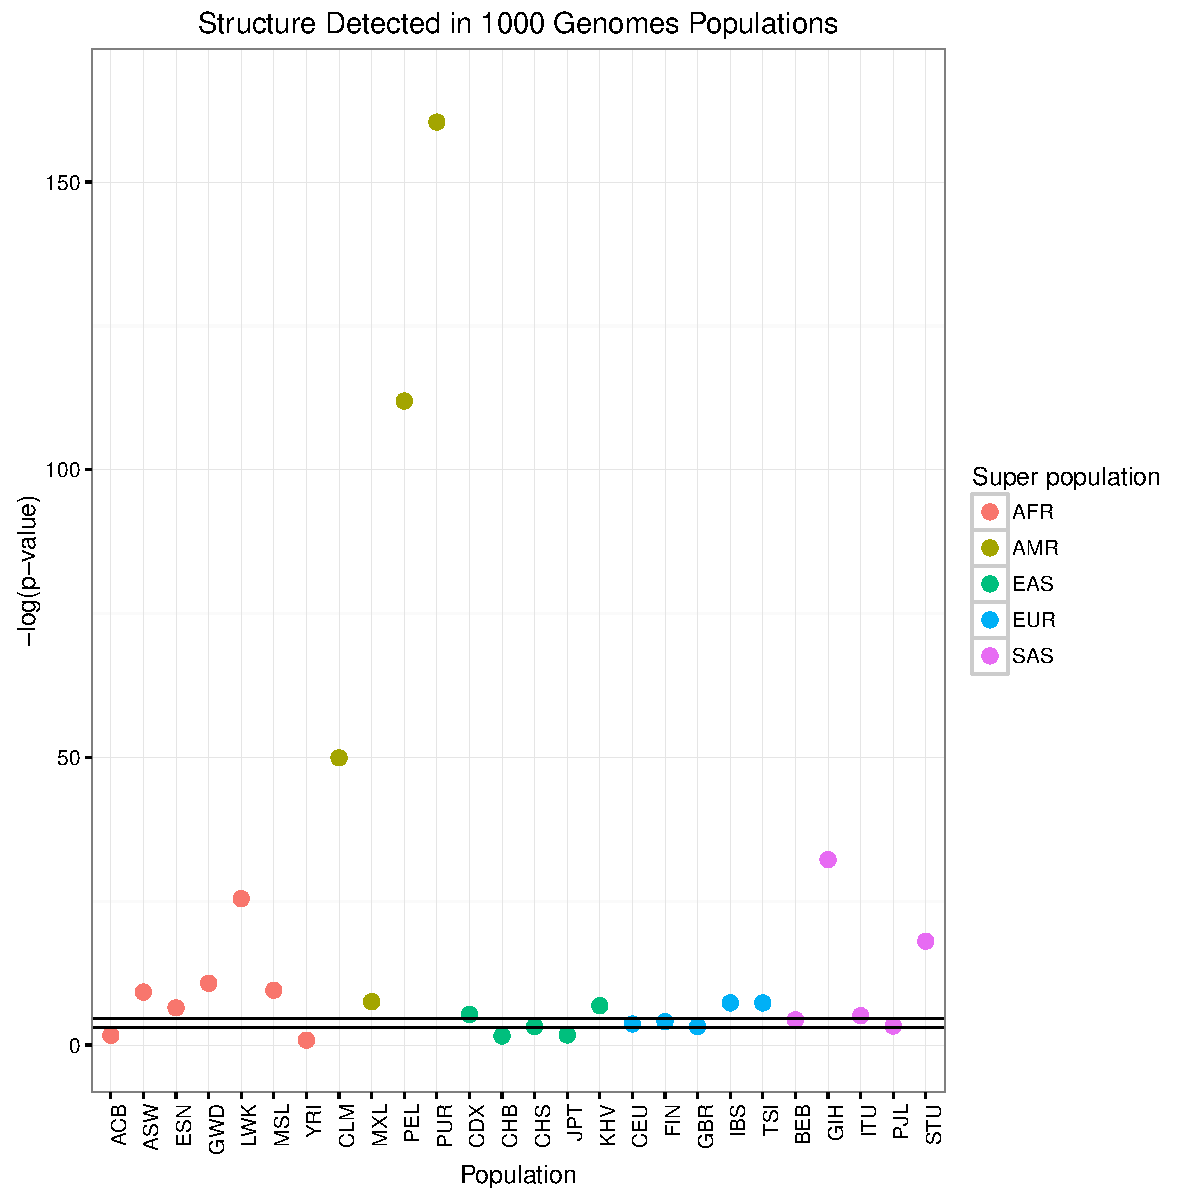
\includegraphics[width=0.5\columnwidth]{figures/PreFilter/pValueForPop}\textbf{B}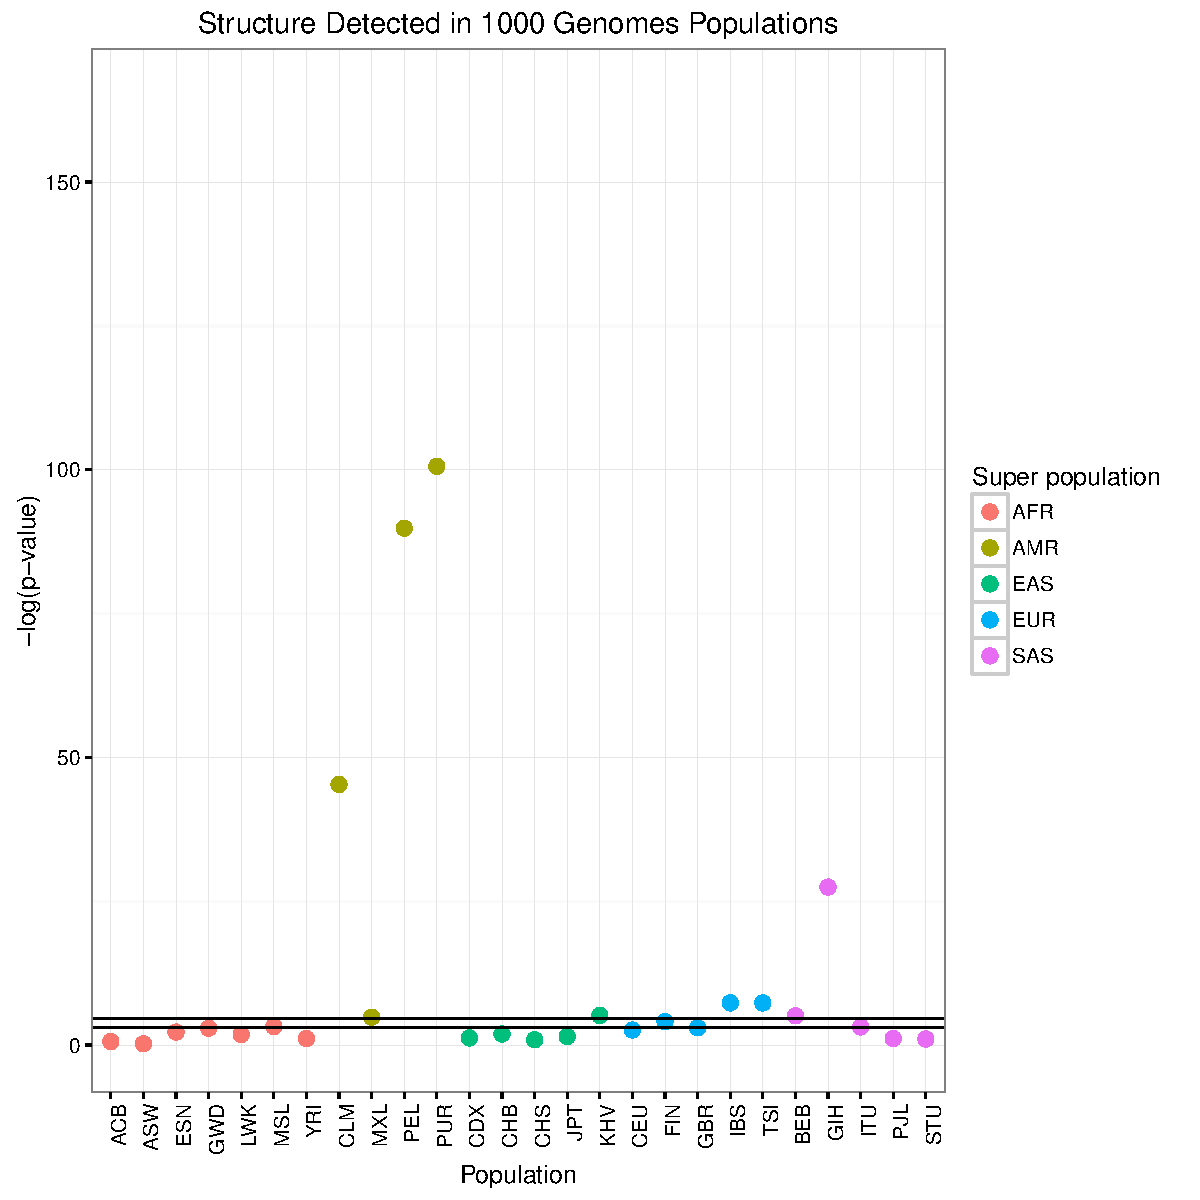
\includegraphics[width=0.5\columnwidth]{figures/PostFilter/pValueForPop}\caption{\textbf{Significance of population heterogeneity in 26 populations
of the TGP}. Detection of population structure was found at $p<.01$
in 15 of the 26 populations using the full dataset (A). Upon removal
of suspected related individuals, four populations (CLM, PEL, PUR
and GIH) violated homogeneity in the relatedness-removed populations
(B).}
\label{fig: Structure pvals}
\end{figure}

\begin{figure}
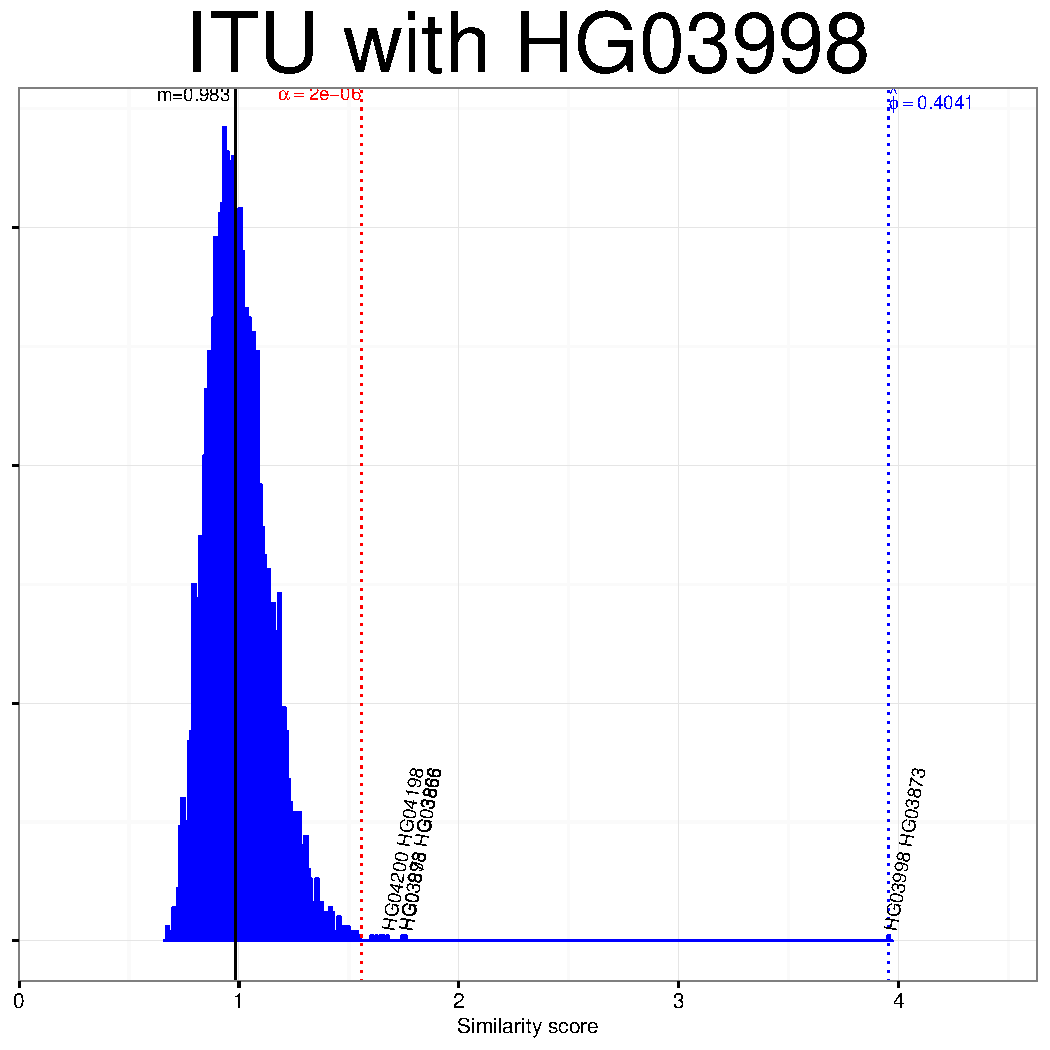
\includegraphics[width=0.4\columnwidth]{figures/ITU_with_HG03998}\caption{Distribution of all pairwise $s$ statistics for population Indian
Telugu from the UK (ITU) with individual HG03998 included. HG03998
is now believed to be related to HG03873, despite being labeled in
the Sri Lankan Tamil from the UK (STU) population. The family-wise
$\alpha=.01$ cutoff is indicated by the dotted red vertical line
and the $s$ statistic for HG03998 and HG03873 is seen as an extreme
outlier at 3.97.}
\label{fig: ITU with HG03998}
\end{figure}

\begin{figure}
\textbf{Distribution of similarity statistic within population subgroups
from 1000 Genomes Project }

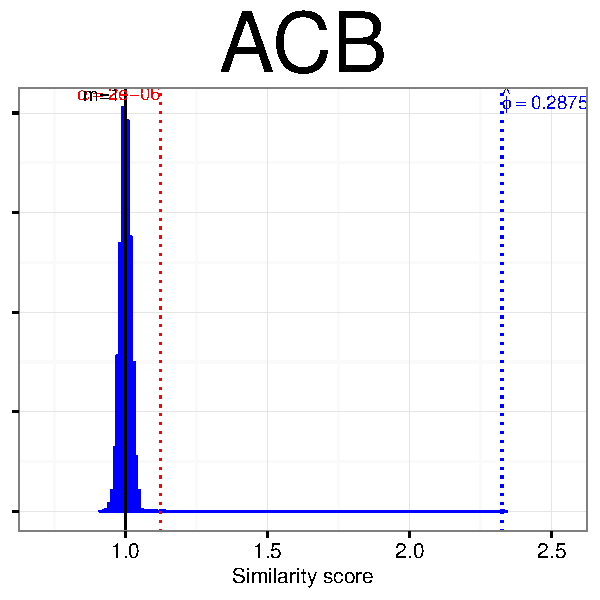
\includegraphics[width=0.12\paperwidth]{figures/PreFilter/ACBdiploid}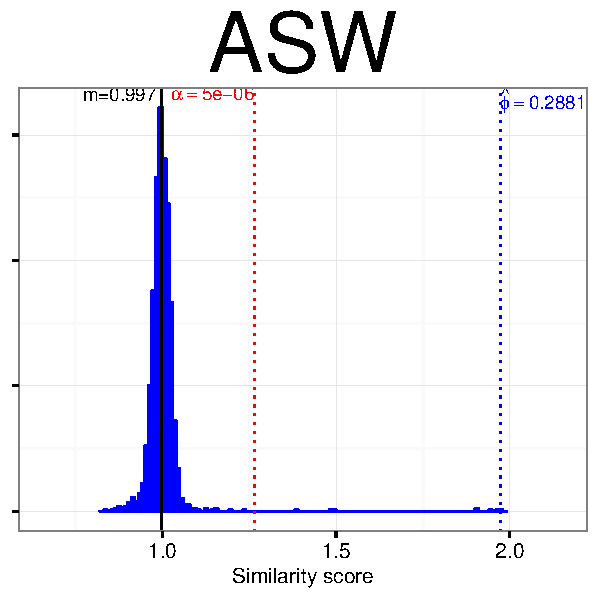
\includegraphics[width=0.12\paperwidth]{figures/PreFilter/ASWdiploid}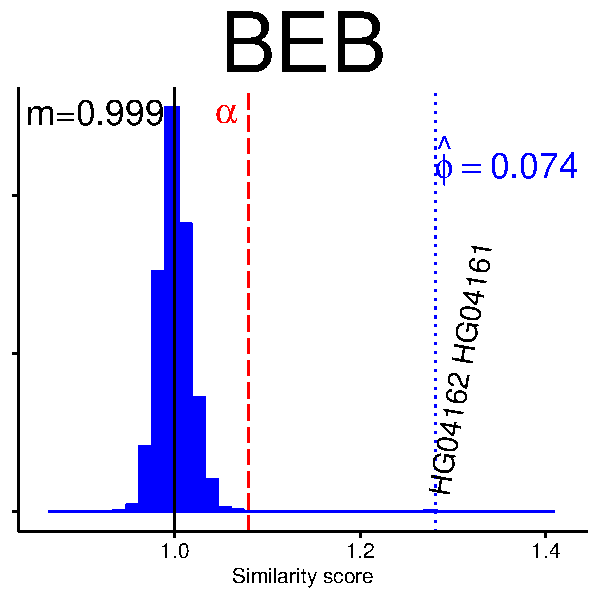
\includegraphics[width=0.12\paperwidth]{figures/PreFilter/BEBdiploid}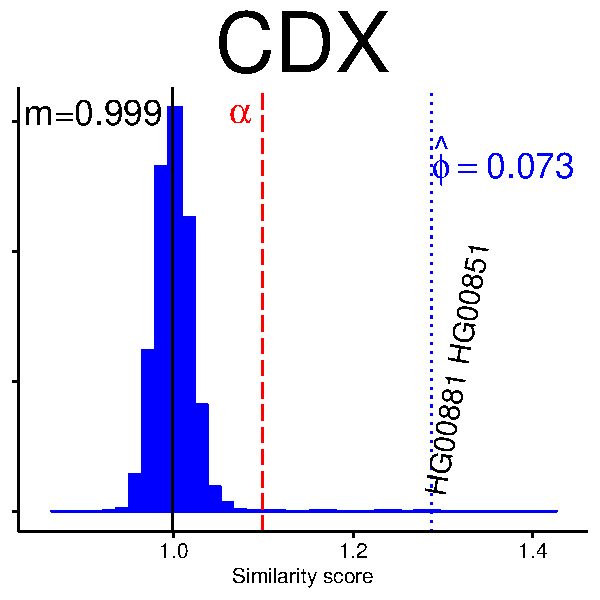
\includegraphics[width=0.12\paperwidth]{figures/PreFilter/CDXdiploid}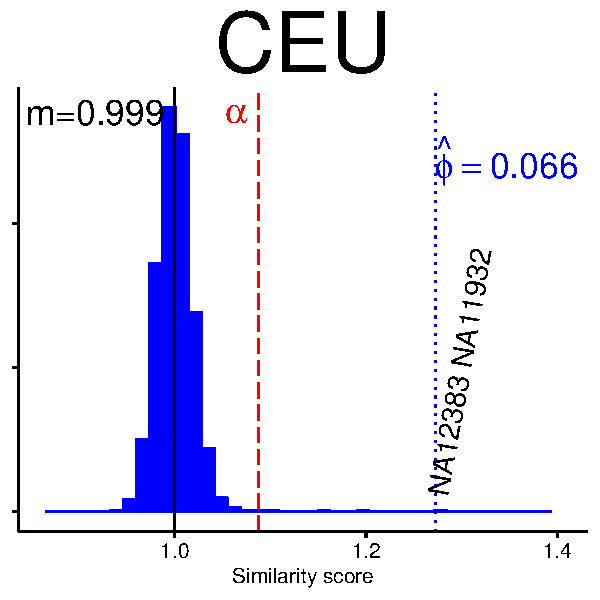
\includegraphics[width=0.12\paperwidth]{figures/PreFilter/CEUdiploid}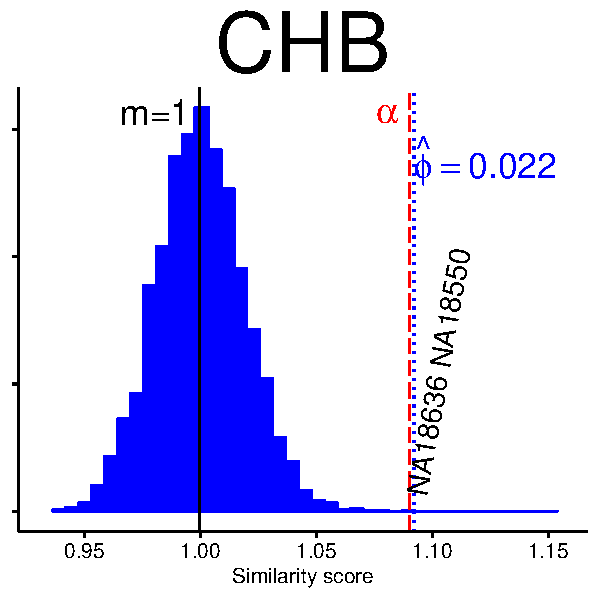
\includegraphics[width=0.12\paperwidth]{figures/PreFilter/CHBdiploid}

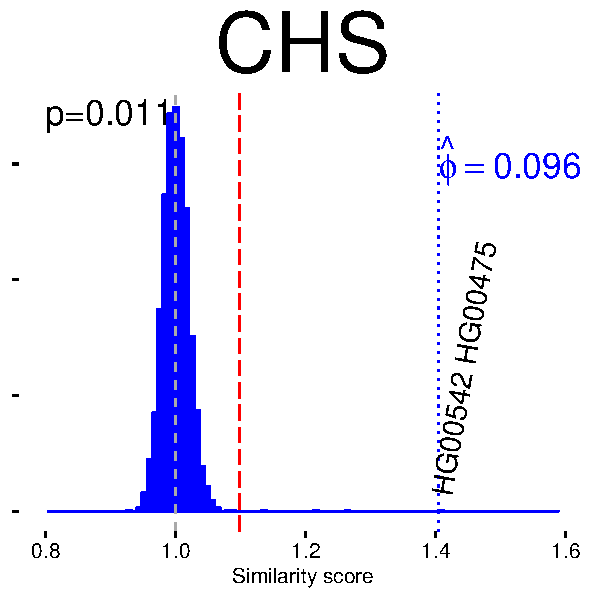
\includegraphics[width=0.12\paperwidth]{figures/PreFilter/CHSdiploid}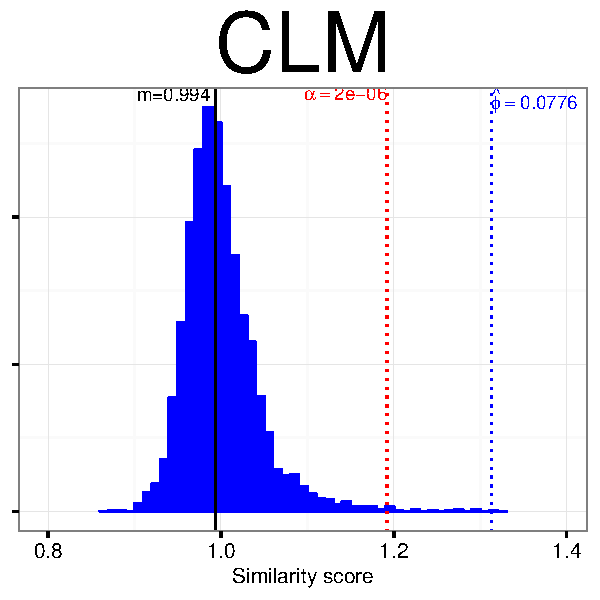
\includegraphics[width=0.12\paperwidth]{figures/PreFilter/CLMdiploid}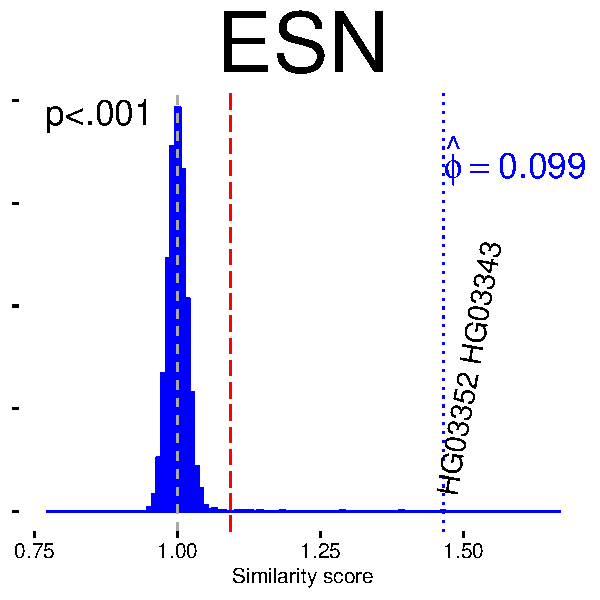
\includegraphics[width=0.12\paperwidth]{figures/PreFilter/ESNdiploid}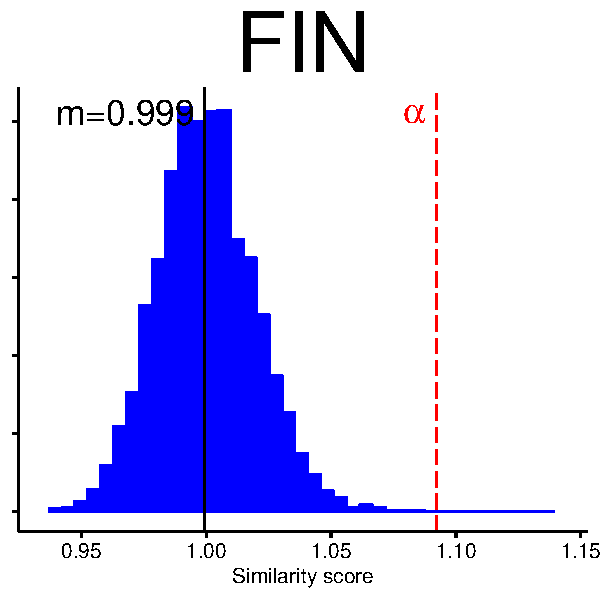
\includegraphics[width=0.12\paperwidth]{figures/PreFilter/FINdiploid}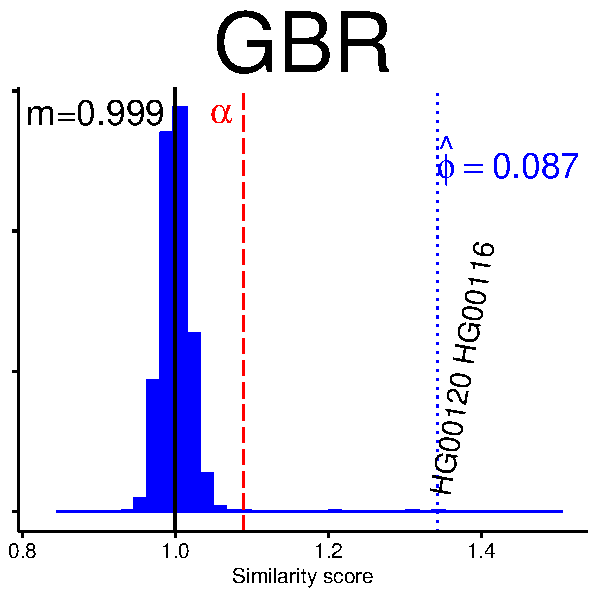
\includegraphics[width=0.12\paperwidth]{figures/PreFilter/GBRdiploid}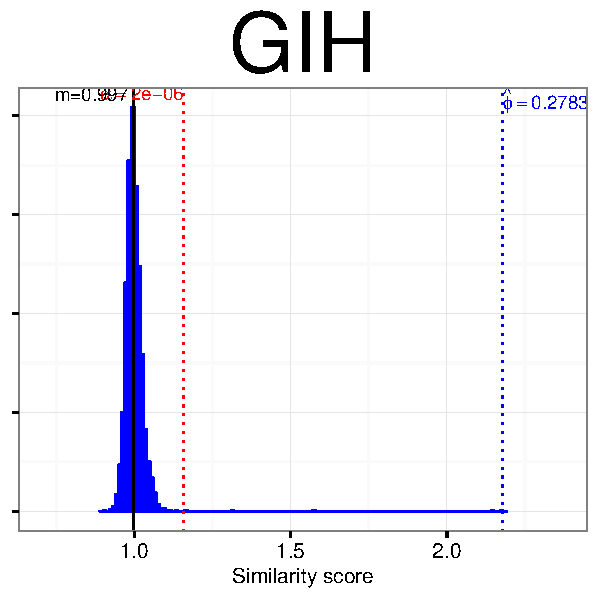
\includegraphics[width=0.12\paperwidth]{figures/PreFilter/GIHdiploid}

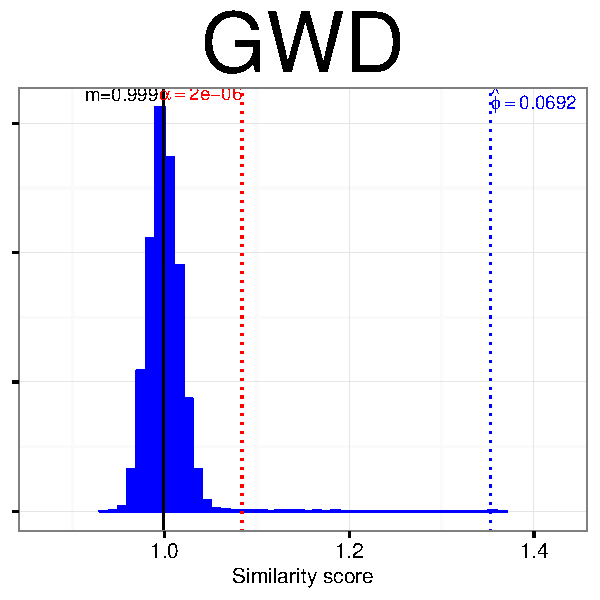
\includegraphics[width=0.12\paperwidth]{figures/PreFilter/GWDdiploid}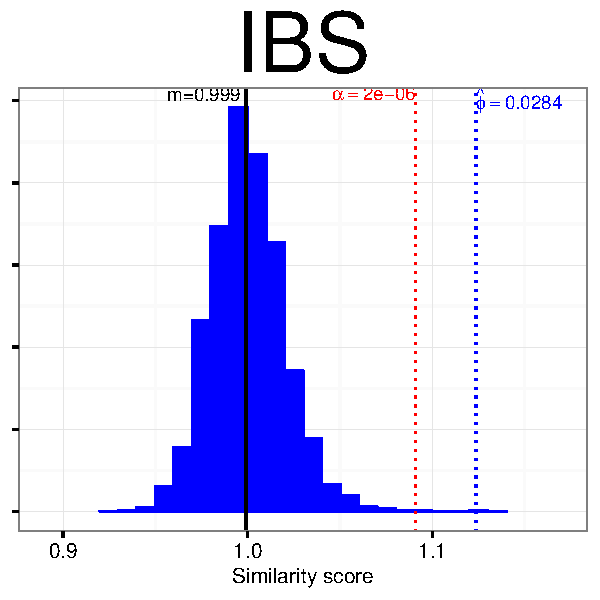
\includegraphics[width=0.12\paperwidth]{figures/PreFilter/IBSdiploid}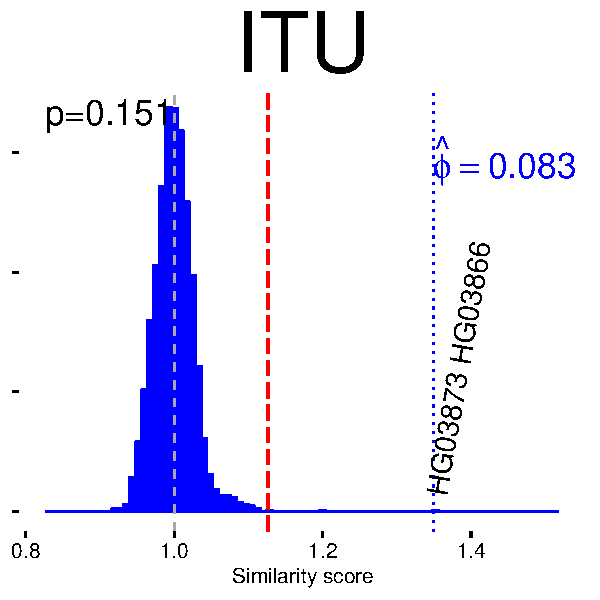
\includegraphics[width=0.12\paperwidth]{figures/PreFilter/ITUdiploid}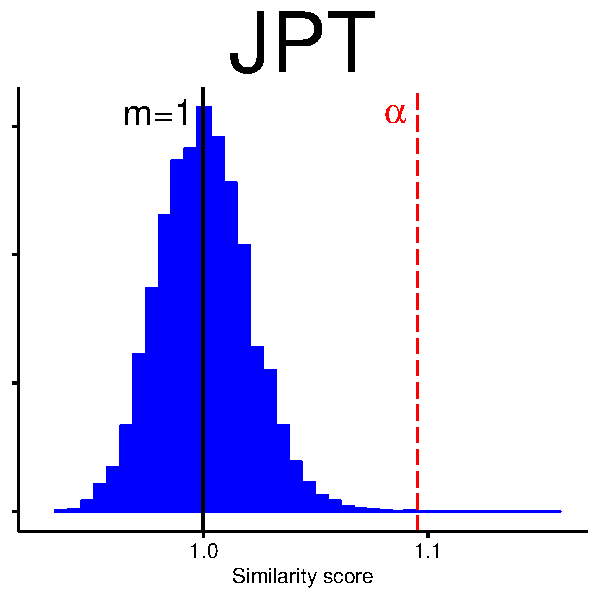
\includegraphics[width=0.12\paperwidth]{figures/PreFilter/JPTdiploid}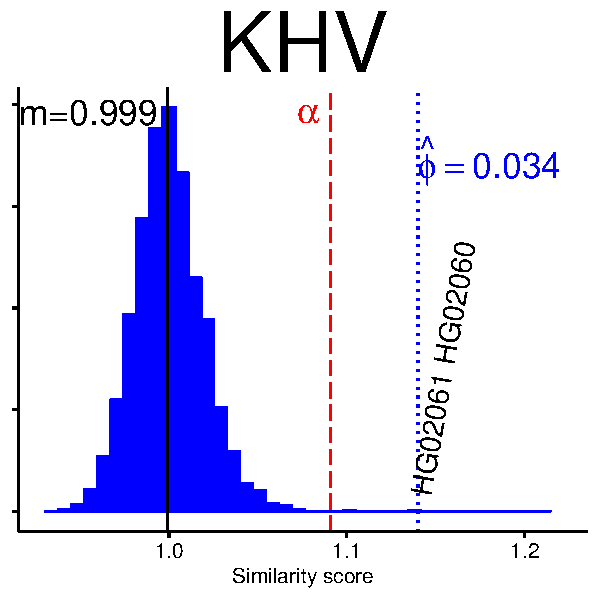
\includegraphics[width=0.12\paperwidth]{figures/PreFilter/KHVdiploid}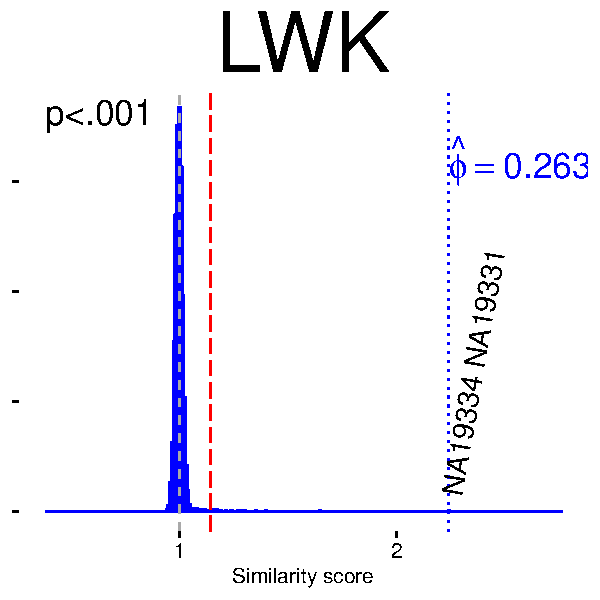
\includegraphics[width=0.12\paperwidth]{figures/PreFilter/LWKdiploid}

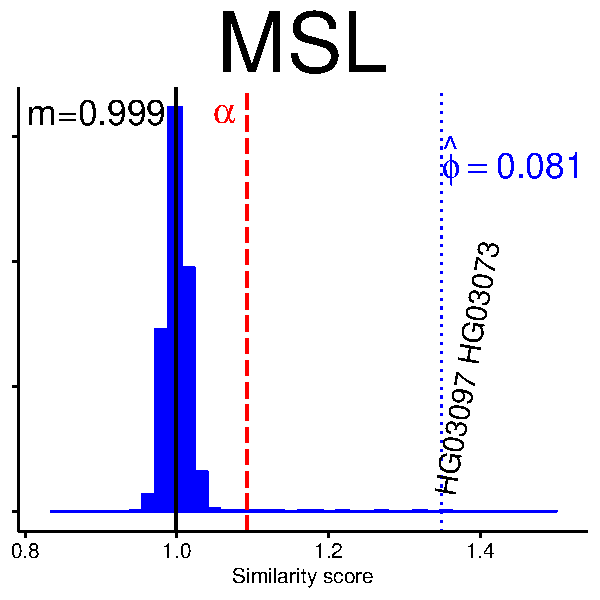
\includegraphics[width=0.12\paperwidth]{figures/PreFilter/MSLdiploid}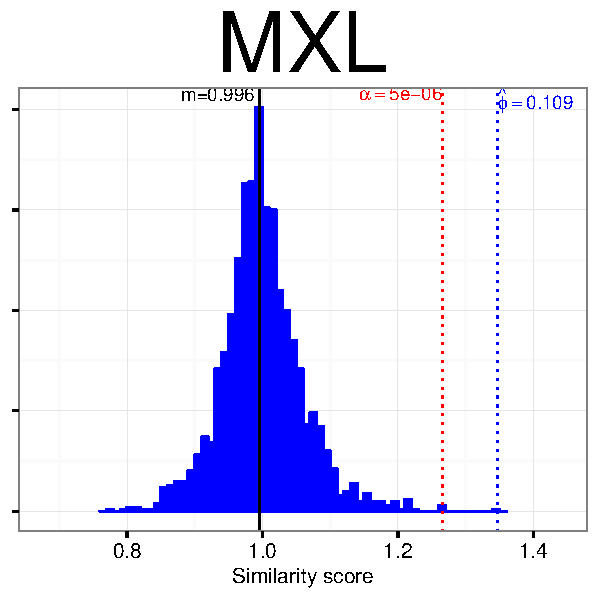
\includegraphics[width=0.12\paperwidth]{figures/PreFilter/MXLdiploid}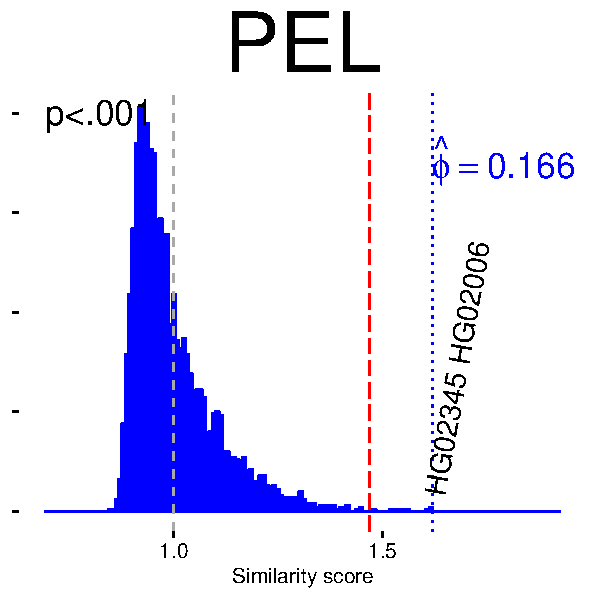
\includegraphics[width=0.12\paperwidth]{figures/PreFilter/PELdiploid}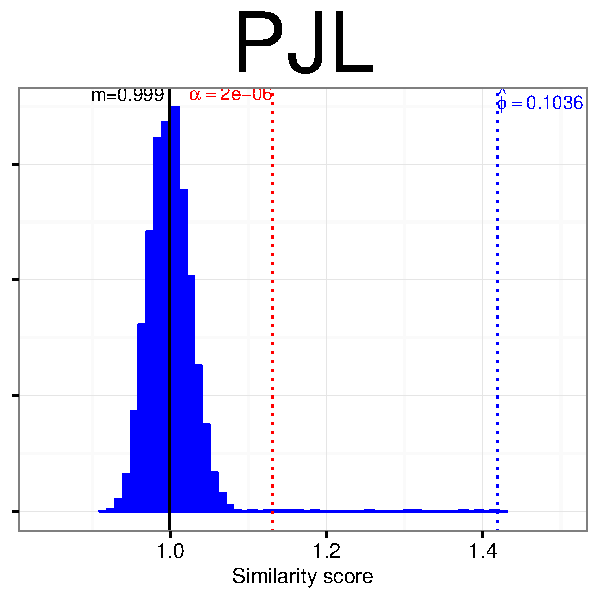
\includegraphics[width=0.12\paperwidth]{figures/PreFilter/PJLdiploid}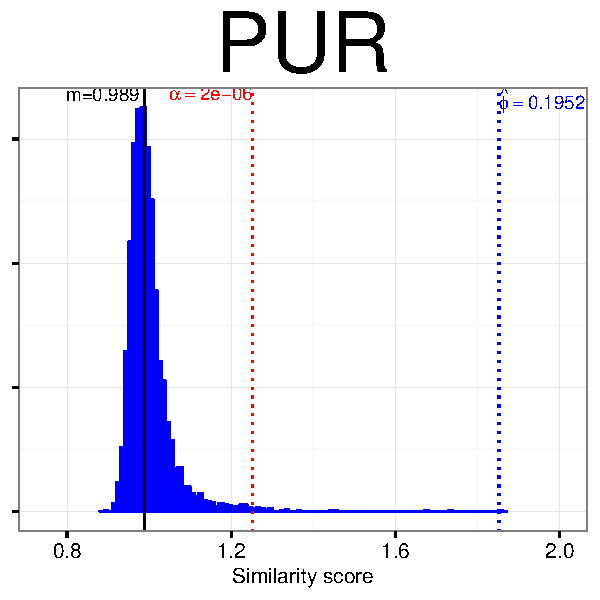
\includegraphics[width=0.12\paperwidth]{figures/PreFilter/PURdiploid}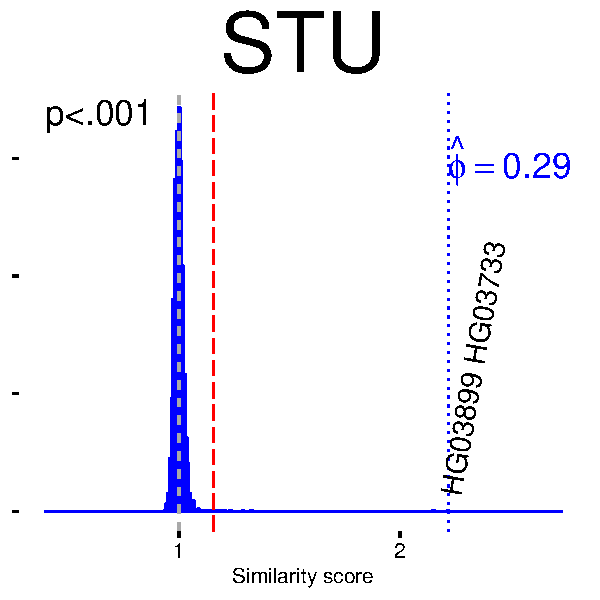
\includegraphics[width=0.12\paperwidth]{figures/PreFilter/STUdiploid}

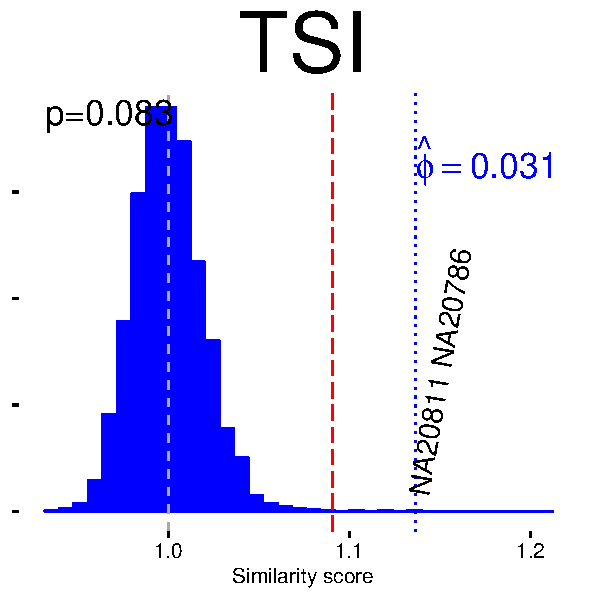
\includegraphics[width=0.12\paperwidth]{figures/PreFilter/TSIdiploid}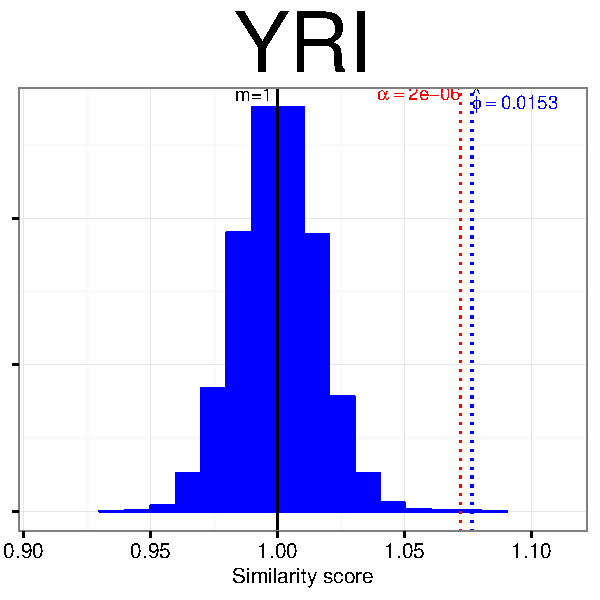
\includegraphics[width=0.12\paperwidth]{figures/PreFilter/YRIdiploid}\caption{Distribution of similarity coefficients for each of the 26 populations
in the 1000 Genomes Project. Homogeneous populations lacking cryptic
relatedness should be expected to exhibit distributions centered around
1 with no outliers. The red dotted vertical line on each plot indicates
the family-wise$\alpha=.01$ level cutoff for ${n \choose 2}$ comparisons.
The most significant related pair is labeled for each population with
the estimated kinship for that pairing indicated in blue. The p-value
for the KS test for homogeneity is reported for each population. Many
of the population groups do demonstrate the null behavior (e.g. JPT,
KHV, FIN), however, a number of populations show the presence of extreme
outliers (e.g. STU, PUR) or systematic right skew (e.g. MXL, PEL)}
\label{fig: All s plots}
\end{figure}

\begin{table}
\begin{tabular}{|c|c|c|c|}
\hline 
Population & Super Population & Structure & Cryptic Relatedness\tabularnewline
\hline 
\hline 
ACB & \multirow{7}{*}{AFR - African} & NO & NO\tabularnewline
\cline{1-1} \cline{3-4} 
ASW &  & NO & \textbf{YES}\tabularnewline
\cline{1-1} \cline{3-4} 
ESN &  & NO & NO\tabularnewline
\cline{1-1} \cline{3-4} 
GWD &  & NO & NO\tabularnewline
\cline{1-1} \cline{3-4} 
LWK &  & NO & NO\tabularnewline
\cline{1-1} \cline{3-4} 
MSL &  & NO & NO\tabularnewline
\cline{1-1} \cline{3-4} 
YRI &  & NO & YES\tabularnewline
\hline 
CLM & \multirow{4}{*}{AMR - Ad Mixed American} & \textbf{YES} & \textbf{YES}\tabularnewline
\cline{1-1} \cline{3-4} 
MXL &  & NO & NO\tabularnewline
\cline{1-1} \cline{3-4} 
PEL &  & \textbf{YES} & \textbf{YES}\tabularnewline
\cline{1-1} \cline{3-4} 
PUR &  & \textbf{YES} & \textbf{YES}\tabularnewline
\hline 
CDX & \multirow{5}{*}{EAS - East Asian} & NO & NO\tabularnewline
\cline{1-1} \cline{3-4} 
CHB &  & NO & NO\tabularnewline
\cline{1-1} \cline{3-4} 
CHS &  & NO & NO\tabularnewline
\cline{1-1} \cline{3-4} 
JPT &  & NO & NO\tabularnewline
\cline{1-1} \cline{3-4} 
KHV &  & NO & NO\tabularnewline
\hline 
CEU & \multirow{5}{*}{EUR - European} & NO & NO\tabularnewline
\cline{1-1} \cline{3-4} 
FIN &  & NO & NO\tabularnewline
\cline{1-1} \cline{3-4} 
GBR &  & NO & NO\tabularnewline
\cline{1-1} \cline{3-4} 
IBS &  & NO & NO\tabularnewline
\cline{1-1} \cline{3-4} 
TSI &  & NO & NO\tabularnewline
\hline 
BEB & \multirow{5}{*}{SAS - South Asian} & NO & NO\tabularnewline
\cline{1-1} \cline{3-4} 
GIH &  & \textbf{YES} & NO\tabularnewline
\cline{1-1} \cline{3-4} 
ITU &  & NO & NO\tabularnewline
\cline{1-1} \cline{3-4} 
PJL &  & NO & NO\tabularnewline
\cline{1-1} \cline{3-4} 
STU &  & NO & NO\tabularnewline
\hline 
\end{tabular}\caption{\textbf{Presence of population structure and cryptic relatedness detected
in each of the 26 populations in the 1000 Genomes Project.} STEGO
was run separately on each population group following the removal
of suspected related individuals. Population structure was defined
as a significant $\left(p<.01\right)$ Kolmogorov-Smirnov statistic
comparing the observed test statistic distribution to that expected
under the assumption of homogeneity. Cryptic relatedness was defined
as those populations containing at least one pair of individuals with
estimated kinship $\hat{\phi}>\frac{1}{32}$ and statistically significant
$\left(p<.01\right)$ kinship after multiple testing correction. }

\label{population_table}
\end{table}


\subsection*{Population differentiation in 1000 Genomes Project}

There are many methods for detecting population structure. Most commonly,
Principal Components Analysis \cite{price2006principal,price2010new}
is applied for identifying the components of largest variation which
ideally corresponds to the population structure. This procedure first
involves the calculation of a genetic similarity matrix (GSM) via
the correlation between all samples, which is commonly followed by
an eigendecomposition of that matrix. There are a number of limitations
to this straightforward approach, one of which is that the calculation
of a variance-covariance matrix equally weights the impact of all
loci, failing to fully utilize the fact that the overall allele frequency
is informative of the value of each variant. Recently, the use of
the Jaccard Index has been used to estimate genetic similarity\cite{prokopenko2016utilizing}.
This approach provides a higher resolution picture of the genetic
landscape by exploiting the co-occurrence of rare-variants in sequencing
data. STEGO directly utilizes this the differential value of alleles
based on minor allele frequency by weighting variants by how unlikely
such a co-occurrence would have been in a homogeneous population. 

We evaluated the effectiveness of our similarity measure to differentiate
populations in the TGP in both global and localized contexts. For
the global scenario we used data from all 26 populations in a single
analysis. In the localized scenarios, we ran 57 separate analyses
corresponding to all possible pairs of populations within each of
the five superpopulations. In each analysis, STEGO was used to compute
the GSM containing all pairwise similarity scores. An eigendecomposition
of the GSM was performed and each individual in the study was plotted
against the top two eigenvectors. 

In comparing our results with those of PCA, we achieve highly similar
results on the global scale depicting the two dimensional linear migrations
of ancient human history. However, despite a focus on separating recently
related populations, STEGO is effective at partitioning samples of
more distant common ancestry as well (Figure \ref{fig: heatmaps}). 

\begin{figure}
\textbf{A}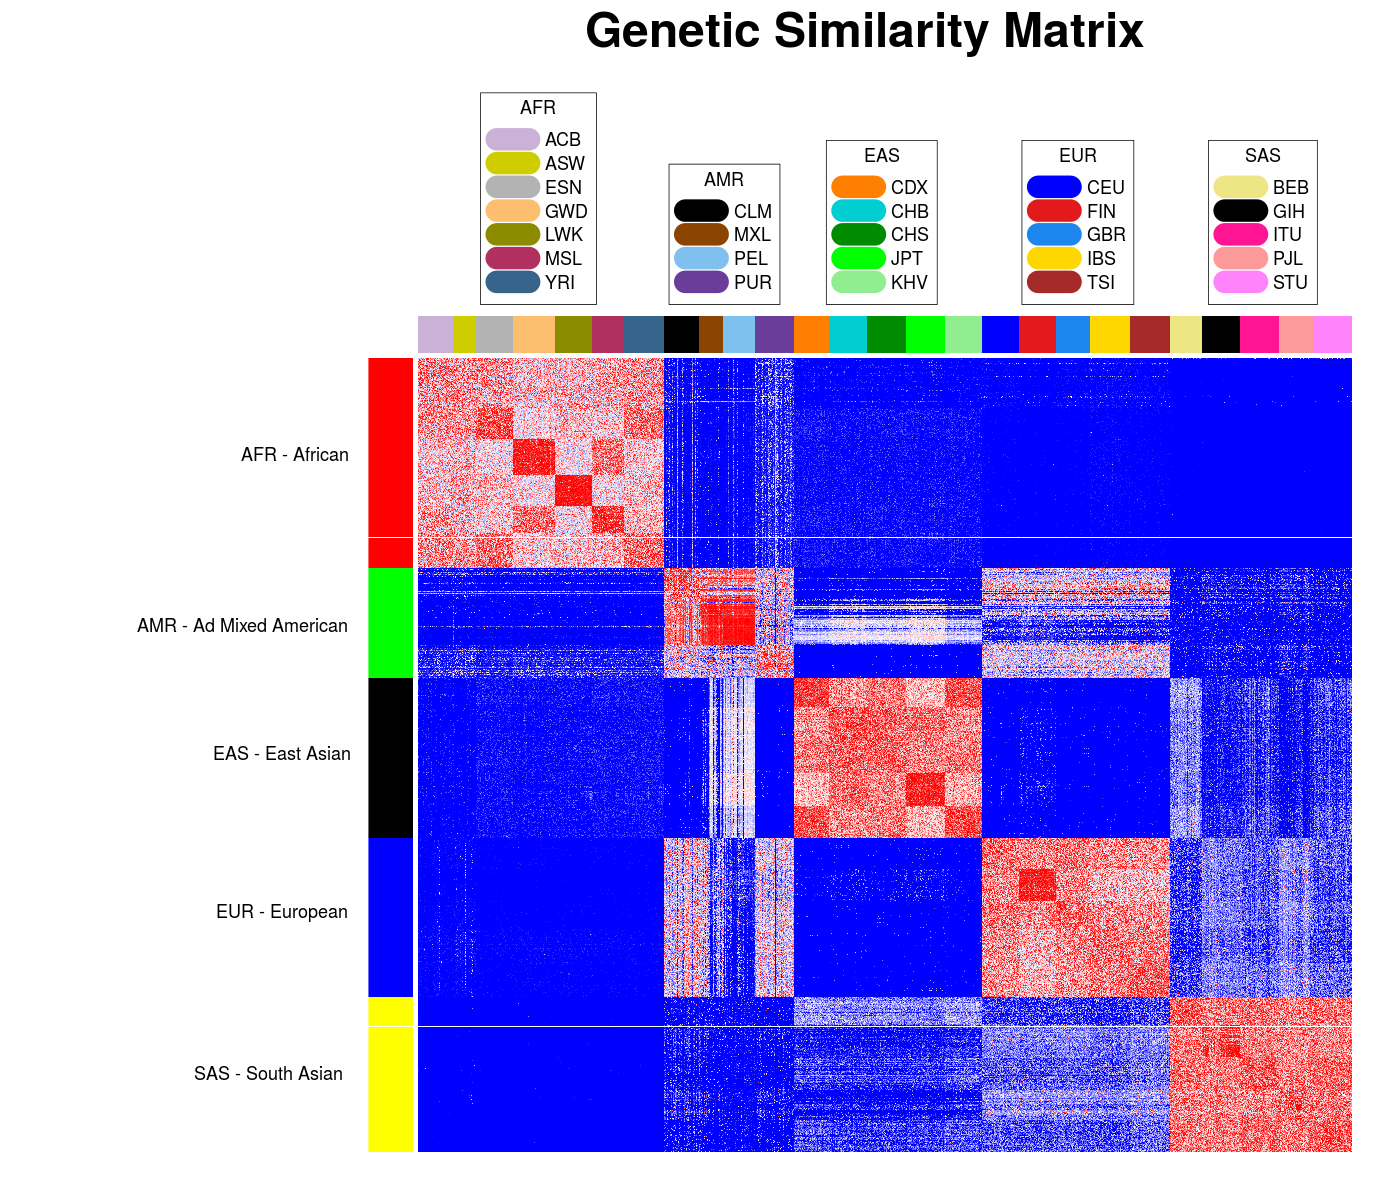
\includegraphics[width=0.9\columnwidth]{figures/GSM}

\textbf{B}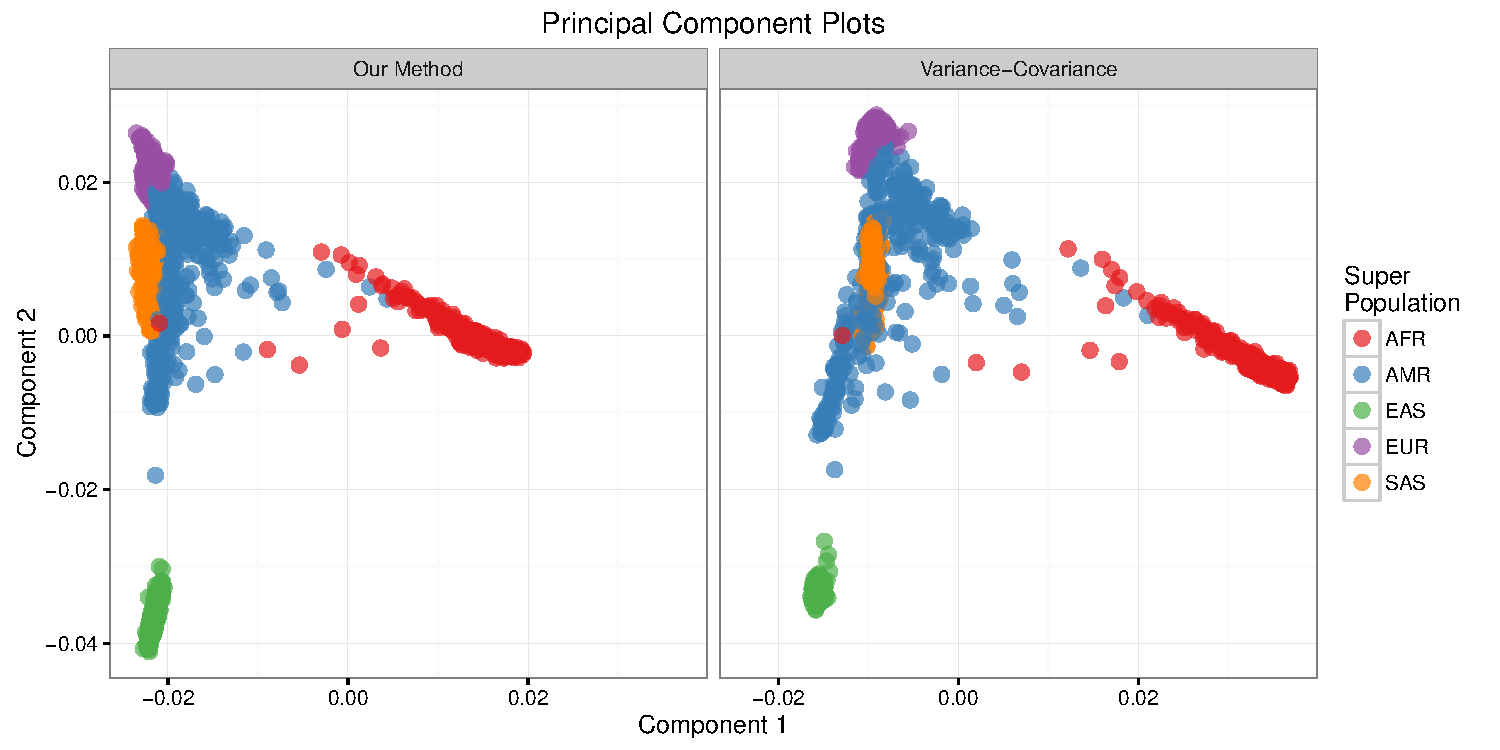
\includegraphics[width=1\columnwidth]{figures/PCA_all}\caption{Population structure in 2504 samples from 1000 Genomes Project. (\textbf{A})
Heatmap of the GSM generated by STEGO using 80,000 LD-sampled variants.
The vertical colorbar indicates membership in one of the five superpopulations,
while the horizontal colorbar indicates membership in one of the 26
populations. (\textbf{B}) Projecting each individual onto the top
two eigenvectors resulted in a similar 2-dimensional distribution
of global ancestry. Both STEGO and PCA show similar projections which
elucidate the migratory patterns of early humans.}
\label{fig: heatmaps}
\end{figure}

Despite no loss of performance on the global scale, the approach we
describe here outperforms standard PCA when the task involves classifying
individuals of recent ancestry. Focusing only on populations belonging
to the same continental super-population, every possible pair was
merged following the removal of suspected related pairs. STEGO and
standard PCA were then run on each merged dataset and the two methods
were compared by computing the ratio of mean within-population variance
to total variance across the first three principal components. 

The results show that STEGO outperforms PCA by this measure in 41
of the 57 possible comparisons (binomial test $p<.001$) (Supplementary
Figure S2). We chose a pair of closely related populations from the
1000 Genomes Project in order to demonstrate this performance. The
populations Sri Lankan Tamil (STU) and Indian Telugu (ITU) have relatively
small geographical separation and recent common ancestry relative
to other populations in the TGP. We used a subset of each population
determined to be homogeneous and lacking cryptic relatedness as described
above. We demonstrate the clearer separation in (Figure \ref{fig: ITUvsSTU})
comparing our method with that of standard Principal Components Analysis.

The reasoning behind the superior performance in fine scale population
stratification is due to the focus on rarer alleles. Rare alleles
tend to be less stable over generations and become fixed at 0\% with
high probability. Therefore, rare alleles that are observed are more
likely to have arisen recently. It stands to reason that these alleles
would therefore be the most informative of recently related populations.
By appropriately recognizing the increased information contained in
the co-occurrences of less frequent alleles, we achieve superior separation
of recently related populations.

\begin{figure}
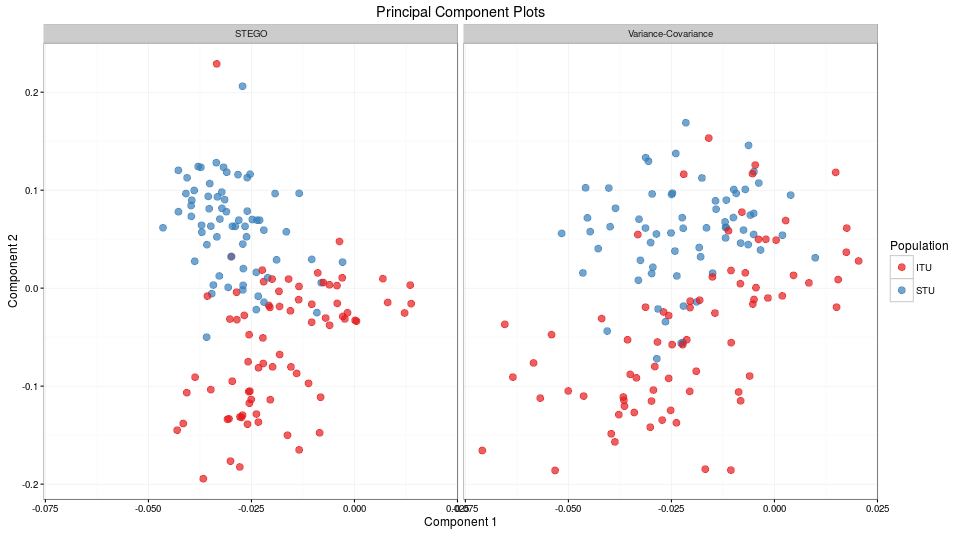
\includegraphics[width=0.8\columnwidth]{figures/PCA_ITU_STU}\caption{\textbf{Example: ITU vs STU}. Two populations of Southern Asian origin,
Indian Telugu from the UK (ITU) and Sri Lankan Tamil from the UK (STU).
A genetic similarity matrix was computed using STEGO and standard
correlation. An eigendecomposition of each matrix was performed. These
plots show the set of unrelated individuals projected on to the first
two eigenvectors. We see clearer clustering by population (colored)
in our method (Left) compared to standard PCA (right). This performance
boost is attributed to the value added by preferentially considering
genetic agreement in less frequent alleles.}
\label{fig: ITUvsSTU}
\end{figure}


\section*{Discussion}

The ability to identify genetic outliers has well-established utility
in genome-wide association studies. Many existing methods for identification
of genetic associations are predicated on the assumptions that population
homogeneity holds in the study. Checking for violations of these assumptions
typically involves a qualitative assessment without any specific concern
for effect size and power. STEGO provides an analytical approach for
quantitatively assess homogeneity and a formal test for the identification
of cryptic relatedness and population stratification.

Several limitations exist with our approach. First, the method assumes
that the variants are independent. We satisfy this assumption by performing
LD sampling, but in doing so limit the number of informative markers
to less than 100k, potentially omitting much of our data and reducing
our power to detect heterogeneity. Furthermore, one's choice of LD
sampling method will necessarily impact the performance of the method.
Additionally, with respect to the detection of population structure,
we cannot design a uniformly most powerful test for structure due
to the complex nature in which structure can exist.

In spite of these limitations, STEGO provides a formal, interpretable
tool which is directly linked to the kinship coefficient. It provides
a formal statistical test for population substructure, identifying
study subjects which are related and subjects which are genetic outliers
in their assigned population. 

\bibliographystyle{plain}
\bibliography{publications}

\end{document}
